\section{Hubo-Ach: Linux on Hubo}

\begin{figure*}[thpb]
  \centering
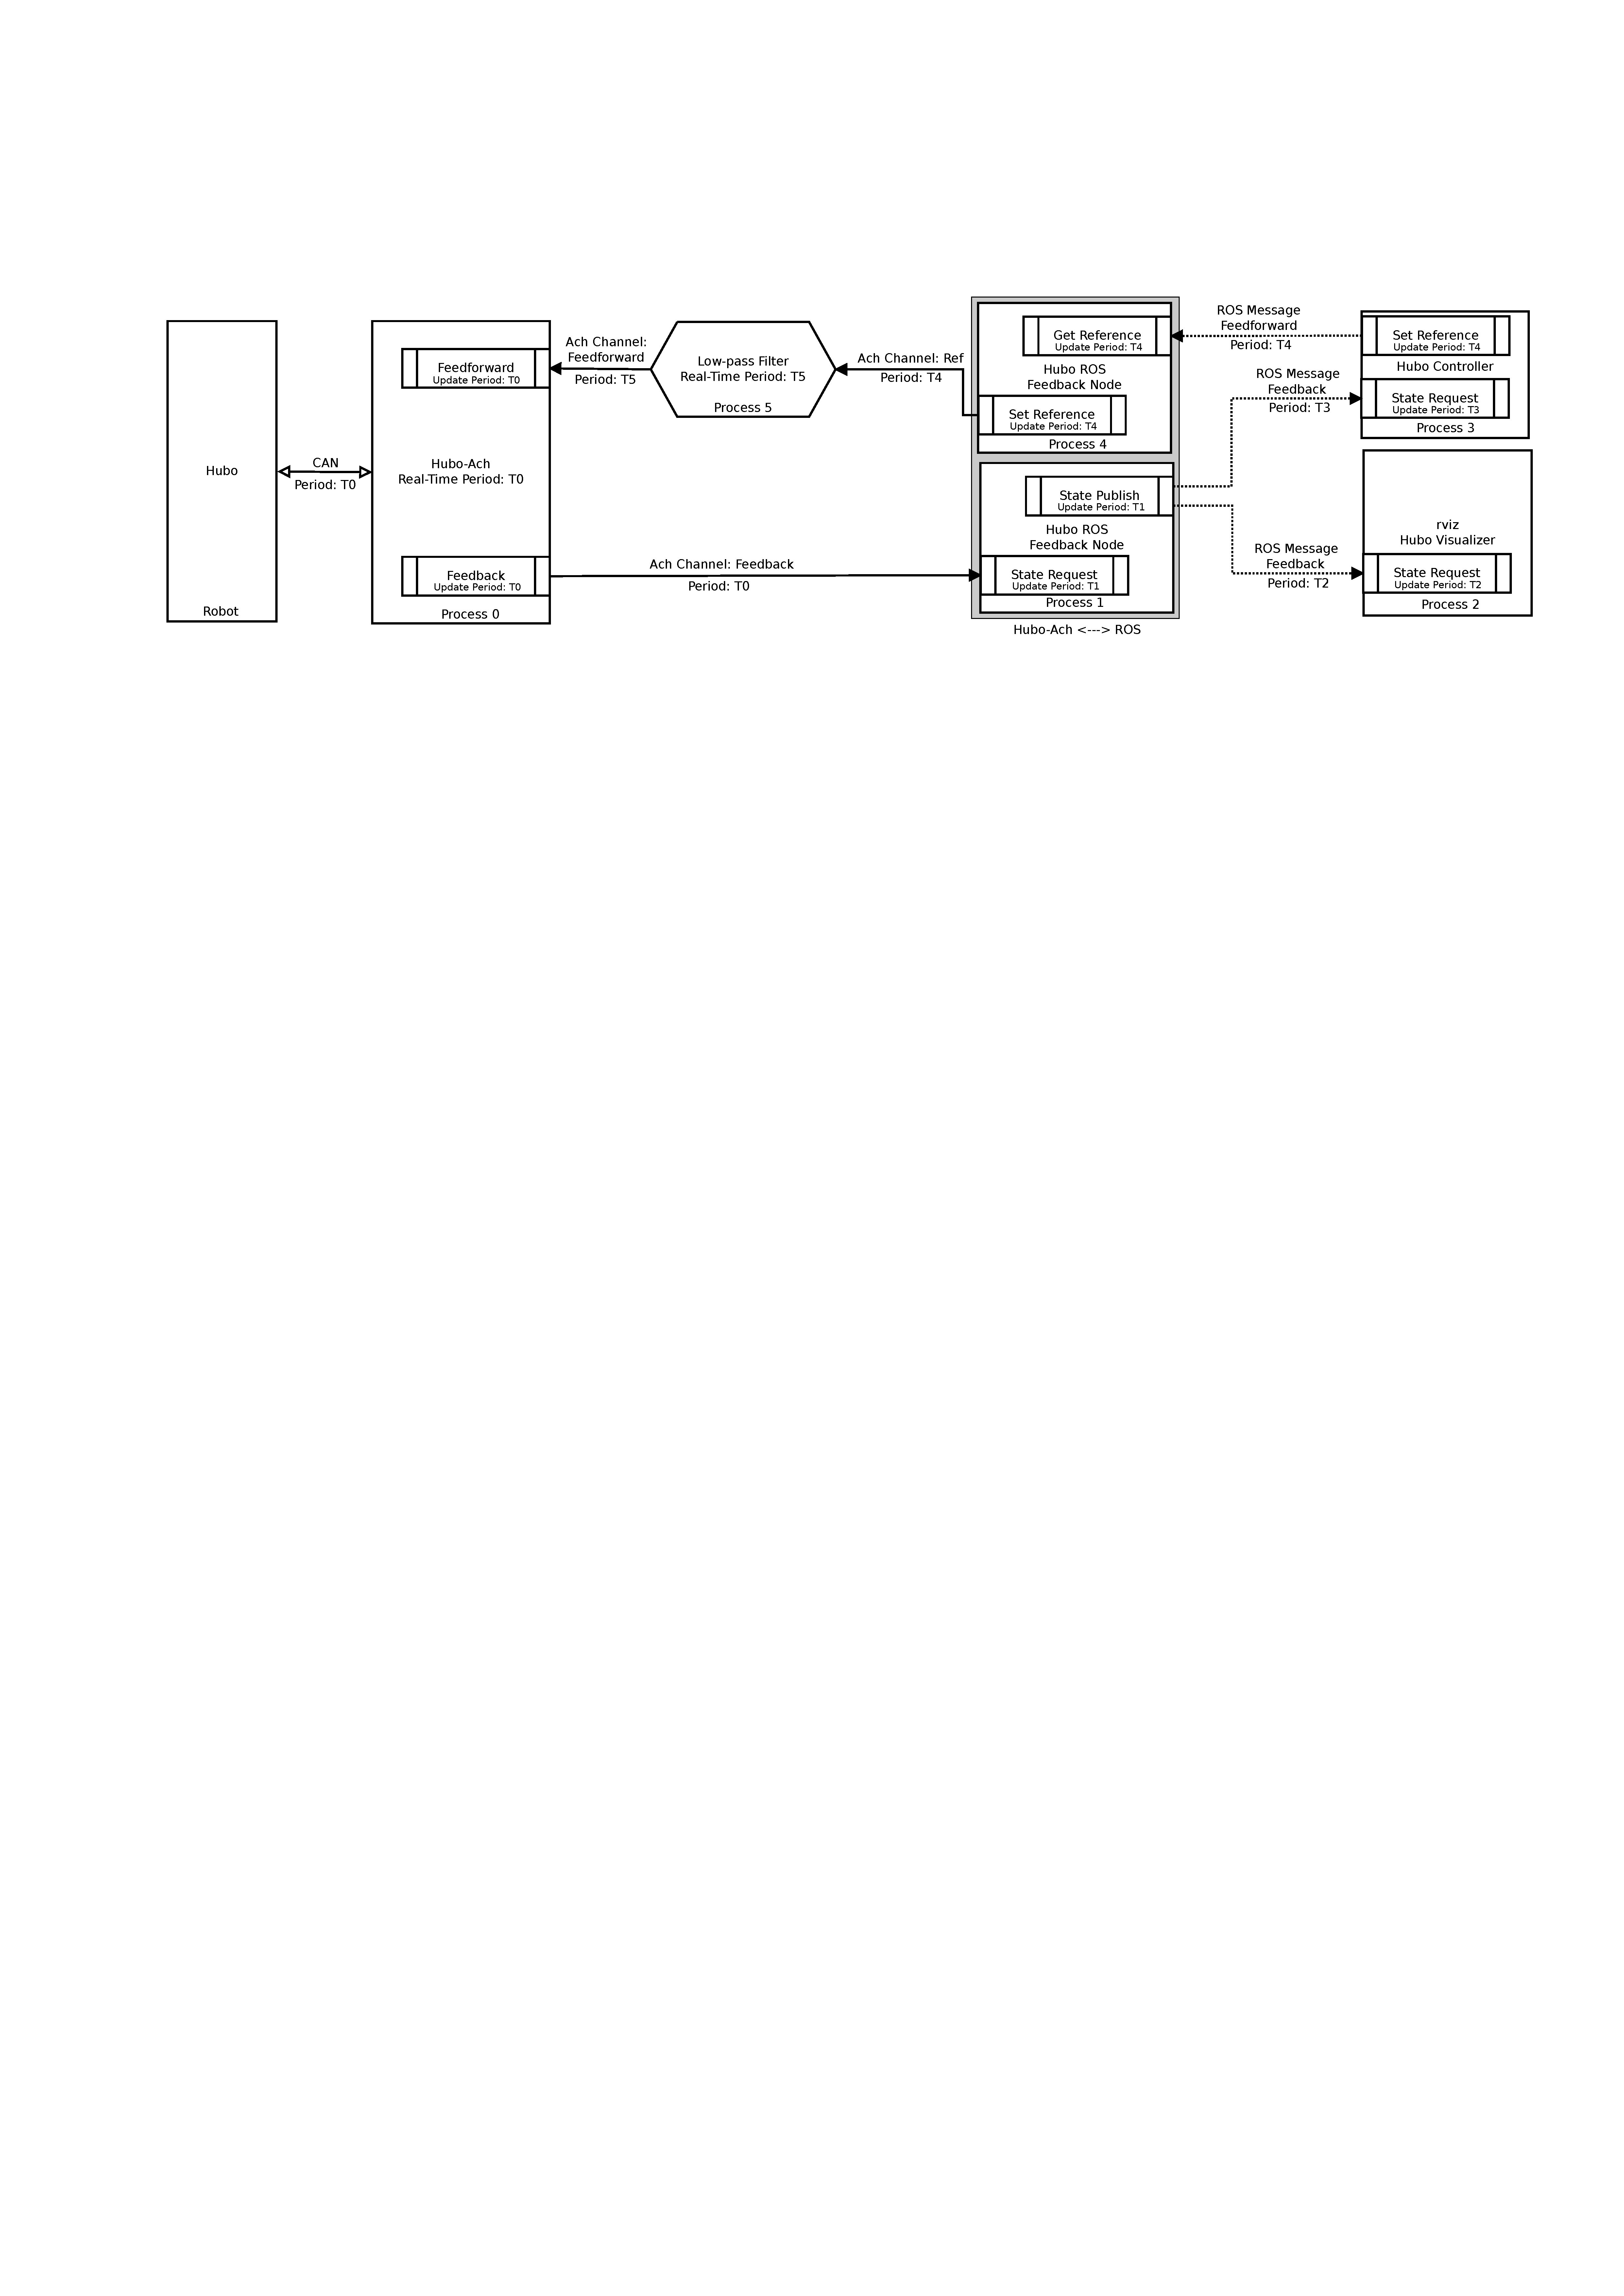
\includegraphics[width=2.0\columnwidth]{./pix/hubo-ach-diagram-ros.pdf}
  \caption{Hubo-Ach interfacing with two seperate processes creating a closed loop system.  Process 0 (Hubo-Ach) takes the most recent command from the Feedforward Ach channel.
  It sends the reference over the CAN bus to the Hubo.  
  The state of the robot is updated and stored in the Feedback Ach chanel.  
  Process 1 reads the state at its own rate, proforms the desired control then sends the the desired references to Process 2.  
This process is a low-pass filter that reduces the jerk on each joint.  
It smooths the desired trajectory allowing Process 1 to send step input to any of the joints at any rate. 
The reference command for each joint is set on the Feedforward Ach channel at a regular rate compleating the closed loop system.}
  \label{fig:graph-ros}
\end{figure*}


Hubo-Ach is the open-source, Linux based, BSD licensed system run on Hubo.  
It was designed by Daniel M. Lofaro\footnote{Daniel M. Lofaro: http://danlofaro.com/} and Neil Dantam and created in collaboration with the \textit{Drexel Autonomous Systems Lab} at Drexel University and \textit{Golems - The Humanoid Robotics Laboratory}\footnote{Golems - The Humanoid Robotics Labatory: www.golems.org/} at the Georgia Institute of Technology.  

The overarching goal of the Hubo-Ach system is to create an easy to use software interface between the Hubo's hardware and the programming environment.  
The design decisions for the system were made with the programmers and developers of the Hubo in mind.
This design philosophy streamlines closed-loop controller implementation, human robot interaction development and the utilization of popular systems such as ROS\footnote{ROS: http://www.ros.org/} (Robot Operating System), OpenRAVE\footnote{OpenRAVE: http://openrave.org/} and MATLAB\footnote{MATLAB: http://www.mathworks.com/} on the Hubo platform.

Hubo-Ach is a daemon process that uses a high-speed, low-latency IPC called Ach \cite{ach} to comunicate with controllers.
Each controller are indipendent processies and are abled to be terminated at anytime without adversly effectling the Hubo-Ach daemon.
Each controller can command the joints at arbritary rates over the Ach channel.
Hubo-Ach impliments a real-time loop in which all of the motor references and state data are set and updated respectively.
The motor references are set via the CAN bus.
At the rising edge of the real-time loop the most recent reference on the feedforward channel is sent.
Sensor updates are requested directly after all references are sent.
The real-time loop runs with a period of $T_0$.
$T_0$ is currently set to 0.005 $sec$.
This causes a CAN bus utiliztion of 78\%.
The real-time loop in Hubo-Ach is needed to ensure the internal phase lock loop (PLL) of the motor controllers lock onto the reference update rate.
This is then used for linear interpolation of the reference onboard the motor controllers.
In addition the real-time is used to ensure no saturation of the CAN bus.
The CAN bus is limited to 1.0 $Mbps$ bandwidth per channel.




Fig.~\ref{fig:graph-ros} shows an example of how the Hubo-Ach system creates a closed-loop system with a Hubo visualizer using ROS and rviz.
\textit{Process 1} and \textit{Process 4} are a part of the Hubo-Ach to ROS layer.
They convert the reference and state data from the Hubo-Ach \textbf{Feedforward} and \textbf{Feedback} channels and convert them to a ROS Message format.
\textit{Process 1} requests feedback data with a period of $T_1$.
If $T_1>T_0$ then \textit{Process 1} will receive the most recent state data received by Hubo-Ach from the Hubo with no overlapping frames.
If $T_1<T_0$ \textit{Process 1} will also receive the latest state data received by Hubo-Ach from the Hubo however some frames will overlap causing identical state data to be returned.
\textit{Process 2} is a Hubo visualizer that is based on the OpenHUBO model \cite{jaemiHuboSRM}.
It reads the Feedback ROS message and shows the commanded joint values and actuial joint values on two seperate Hubo models.
\textit{Process 3} is a controller that reads messages from the ROS Message \textit{Feedback} with a period of $T_3$.
It then proforms a control and posts joint references on the ROS Message \textit{Feedforward} with a period of $T_4$.
The Hubo-Ach to ROS layer on an event based basis. 
As soon as \textit{Process 4} receives a new message posted on the \textit{Feedforward} ROS Message then it posts those same reference values to the Ach Channel \textbf{Ref}.
This means that messages are posted to \textbf{Ref} with a period of $T_4$ which is defined by \textit{Process 3}.
References posted on \textbf{Ref} read by \textit{Process 5} via the \textbf{Ref} Ach channel with an update period of $T_2$.
\textit{Process 2} is a low-pass filter that limits the jerk on each joint.
The resulting trajectory is sent to the \textbf{Feedforward} Ach chanel with a period of $T_3$.
$T_3$ is currently set to 0.01 $sec$.
This means that $T_2$ does not have to be a regular rate.
Thus it is possiable for $T_2>>T3$ with out harm to the robot even it it is a step input.
The resulting movements of Hubo are smooth and jitter free.

The key point is that Hubo-Ach updates the state data in the \textbf{Feedback} Ach channel commands the motors with the references from the \textbf{Feedforward} Ach channel in real-time with a preiod of $T_0$ no matter what rate the external controller is updating the feedforward channel.  
In addition because each controller is its own process, if one of the processes crashes Hubo-Ach does not.
The failed process can then be restarted with no harm done to the robot.




\begin{figure}[thpb]
  \centering
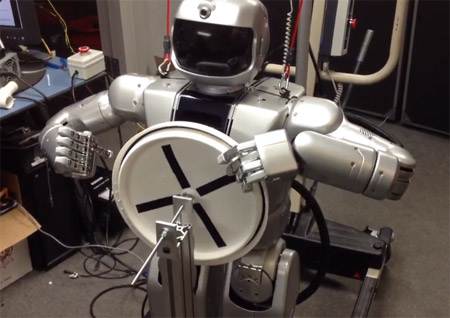
\includegraphics[width=1.0\columnwidth]{./pix/hubo_valve.png}
  \caption{Hubo running PHC turning a valve using trajectories created using Bi-RRTs. }
  \label{fig:valve}
\end{figure}




